\documentclass{beamer}

\usepackage[utf8]{inputenc}
\usepackage[russian]{babel}
\usepackage{amsmath}
\usepackage{beamerthemesplit}
\usetheme[numbers, totalnumbers, compress, nologo]{Statmod}

\title{Алгоритмы и реализация решения задачи сборки ДНК из paired-end данных для сверхбольших геномов}
\author{Владислав Исенбаев}
\institute[СПбНИУ ИТМО]{Санкт-Петербургский национальный исследовательский\\
университет информационных технологий, механики \\
и оптики\\
\vspace{0.4cm}
Научный руководитель: д.т.н., профессор Шалыто~А.~А.}
\date{Санкт-Петербург\\2012 г.}

\begin{document}

\frame{\titlepage}

\section[Содержание]{}
\frame{\tableofcontents}

\section{Исходная задача}
\subsection{Высокопроизводительное секвенирование ДНК}
\frame {
  \frametitle{ДНК}
  Дезоксирибонуклеиновая кислота (ДНК).
  
  \begin{itemize}
  \item Двойная спираль из двух полимерных цепочек.
  \item Составные элементы~--- нуклеотиды.
  \item Комплементарность (A-T, G-C).
  \end{itemize}
}
\frame {
  \frametitle{Метод секвенирования double-ended shotgun} 

  \begin{itemize}
  \item Амплификация исходной ДНК.
  \item Разрезание ДНК на фрагменты.
  \item Выделение фрагментов подходящей длины ($ins=~250$ оснований).
  \item Чтение префикса и суффикса каждого фрагмента (по $n=36$ оснований каждый).
  \item Обработка полученных данных.
  \end{itemize}

  \begin{figure}
    \center{
      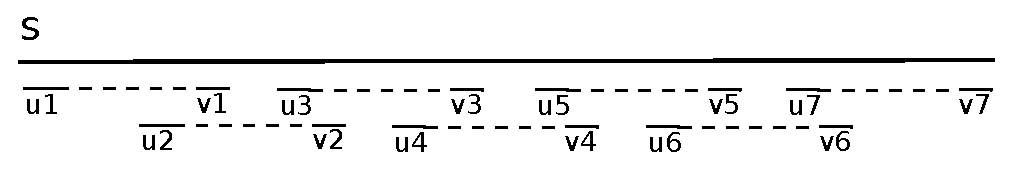
\includegraphics[width=100mm]{../pic/general.svg.eps}
    }
  \end{figure}
}
%\frame {
%  \frametitle{Проблемы}
%  
%  \begin{itemize}
%  \item<1-> Большой объем данных.
%  \item<2-> Ошибки чтения.
%  \item<3-> Полиморфизм.
%  \end{itemize}
%}
%\section{Существующие методы решения задачи}
%\frame{
%  \frametitle{Схема решения}
%  \begin{itemize}
%  \item<1-> Фильтрация ошибок.
%  \item<2-> Решение задачи без использования paired-end данных.
%  \item<3-> Синтез полученных контигов в более длинные последовательности опираясь на paired-end данные.
%  \end{itemize}
%}
\section{Алгоритм восстановления фрагментов}
%\frame{
%  \frametitle{Схема решения}
%  
%  \begin{itemize}
%  \item Фильтрация ошибок.
%  \item Построение сжатого графа де Брейна.
%  \item Удаление ошибочных ветвлений, используя paired-end данные.
%  \item Схлоп полиморфных последовательностей.
%  \item Раскрутка циклов с использованием paired-end данных.
%  \end{itemize}
%}
\frame{
  \frametitle{Описание}
  Построим по исходным данным сжатый граф де Брейна с
  последовательностями в вершинах длиной $k$ .

  \begin{figure}
    \center{
      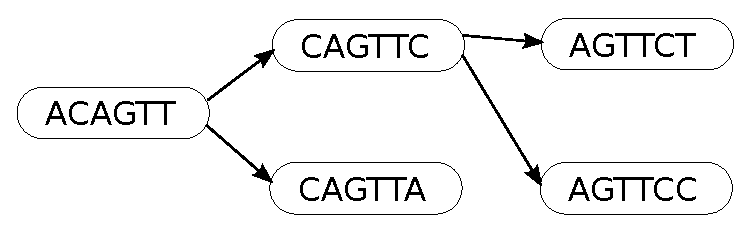
\includegraphics[width=100mm]{../pic/debrujin.svg.eps}
    }
  \end{figure}

  Найдем места в графе, соответствующие началу и концу
  фрагмента. Тогда полным прочтениям фрагмента будут
  соответствовать пути из начального в конечное положение длиной $ins-k$.
}
\frame{
  \frametitle{Оптимизации}
  
  \begin{itemize}
  \item Отсечение по расстоянию до конечной вершины.
  \item Динамическое программирование.
  \end{itemize}
}
\frame{
  \frametitle{Устранение ошибочных ветвлений и разъединение слипшихся
    путей}
  \begin{figure}
    \center{
      \includegraphics[width=100mm]{../pic/unmerge.eps}
    }
  \end{figure}
}
\section{Результаты}
\frame {
  \frametitle{Haemophilus influenzae}
  
Источник данных - симуляция Illumina на референсном геноме
  \begin{itemize}
    \item Размер референс-генома: $1'800'000$ оснований
    \item $100\%$ сборка - $1$ контиг, равный референсной последовательности
    \item Построение графа: $9$ минут на $1$ ноде, $512$ MiB памяти
    \item Сборка: $15$ минут на $1$ нодах, $512$ MiB памяти
  \end{itemize}
}
\frame {
  \frametitle{Escherichia Coli}
  
Данные эксперимента SRR001665
  \begin{itemize}
    \item Размер референс-генома: $4'600'000$ оснований
    \item Покрытие генома контигами: $95\%$
    \item Количество контигов длиннее $100$ оснований: $2'384$
    \item Самый длинный контиг: $35'419$ оснований
    \item $N50=7'800$
    \item Построение графа: $17$ минут на $1$ ноде, $1024$ MiB памяти
    \item Сборка: $18$ минут на $4$ нодах, $256$ MiB памяти на каждой
  \end{itemize}
}
\frame {
  \frametitle{Фрагмент данных dnGASP}
  
Симуляция paired-end чтений без ошибок на
фрагменте тестовых данных dnGASP
  \begin{itemize}
    \item Размер референсного генома: $50'000'000$ оснований
    \item Покрытие генома контигами: $95\%$
    \item Количество контигов длиннее $100$ оснований: $5'012$
    \item Самый длинный контиг: $2'000'370$ оснований
    \item $N50=75'600$
    \item Построение графа: $2$ часов на $4$ нодах, $4096$ MiB памяти
    \item Сборка: $1.5$ часа на $4$ нодах, $2048$ MiB памяти на каждой
  \end{itemize}
}
\frame {
  \frametitle{Drosophila Melanogaster}
  
Данные эксперимента SRR094875
  \begin{itemize}
    \item Референс-геном отсутствует, примерный размер $130'000'000$ оснований
    \item Количество контигов длиннее $100$ оснований: $55'607$
    \item Самый длинный контиг: $112'370$ оснований
    \item $N50=6'600$
    \item Построение графа: $8$ часов на $4$ нодах, $8192$ MiB памяти
    \item Сборка: $6$ часов на $6$ нодах, $2048$ MiB памяти на каждой
  \end{itemize}
}
\section{Вопросы}
\frame {
  \frametitle{Спасибо за внимание!}
  Вопросы?
}
\end{document}
